\chapter{Online Privacy \& Veiligheid}
\label{ch:security}

De informatie in de {\fontseries{extrabold}\selectfont cryptomanual}   \say{{\fontseries{medium}\selectfont best practices}} is bedoeld om mensen te helpen starten met cryptocurrencies. De cryptocurrency-markt is voor velen nog altijd moeilijk toegankelijk en daarom bieden wij hierbij de vereiste basiskennis en hulpmiddelen om dat zowel effectief als veilig te kunnen doen. Aangezien het bezit van cryptocurrency in principe betekent dat je je eigen bank bent, ben jij - en jij alleen - verantwoordelijk voor deze bezittingen.\medskip 

Wie besluit met cryptocurrency te starten, moet dus voldoende aandacht besteden aan online privacy en veiligheid. Een voorselectie is te vinden in dit hoofdstuk. Vergeet niet dat er naast onze suggesties nog vele alternatieve producten bestaan die om welke reden dan ook beter afgestemd kunnen zijn op jouw situatie. Wij geven je enkele handvaten om mee aan de slag te gaan. Kies uit wat voor jou waardevol is en ontdek wat er allemaal nog meer is. Veel dingen zijn gemakkelijk en snel zelf toe te passen - zonder extra kosten. \medskip

\begin{quotation}

      \textit{\say{Bij het beheren van digitale assets - in het bijzonder cryptocurrency vermogen - komt veel eigen verantwoordelijkheid kijken. Jij - en jij alleen - bent verantwoordelijk voor deze eigen investeringen, aangezien er naast de exchange, geen bank, intermediair of andere derde partij bij betrokken hoeft te zijn.}}
      \begin{flushright}
        \small{--- \textbf{cryptomanuals.com}}
      \end{flushright}

\end{quotation}

Elke week worden talloze cryptocurrency gebruikers om allerlei redenen het slachtoffer van verlies en en diefstal van cryptocurrencies. Veel voorkomende redenen zijn dat ze bijvoorbeeld zijn vergeten om 2FA in te schakelen, zwakke wachtwoorden gebruikt hebben of per ongeluk op een phishing link hebben gedrukt.\medskip  

\begin{tipbox}{Tip}
Door onzorgvuldig (online) handelen kan jij blootgesteld worden aan onnodige risico's. Hierdoor is er meer kans dat jouw cryptocurrency in gevaar komt. Wees verstandig en neem het onderwerp online veiligheid en privacy serieus, ook buiten de cryptocurrency wereld om. Wij geven je enkele handvaten om hiermee aan de slag te gaan!    
\end{tipbox}



\section{Risico analyse}
Een risico analyse houdt in dat men kijkt naar de eigen situatie en beoordeeld waar de eventuele risico's liggen. Het klinkt misschien een beetje extreem, maar het kan heel nuttig zijn. Stilstaan bij de risico's die verbonden zijn aan het kopen en verkopen van cryptocurrencies, zorgt ervoor dat er weloverwogen beslissingen worden gemaakt en gebruikers de nodige stappen zetten om zichzelf te beschermen. Hierbij worden alle activiteiten van de gebruiker, investeerder of trader - en de eventuele bijbehorende risico's - onder de loep genomen. 

De meeste nieuwe investeerders zijn zich niet goed bewust van deze risico's. Waar zitten de mogelijke knelpunten in het systeem? Kunnen de cryptocurrencies wel snel worden opgenomen? Is er {\"u}berhaupt toegang tot de eigen crypto? Zijn de keys in eigen beheer? Wat als het e-mailaccount wordt gehacked? Worden overal wel sterke wachtwoorden gebruikt? Door op voorhand over dit soort vragen na te denken, worden de risico's enorm beperkt en voelen investeerders zich veiliger en zelfverzekerder.

\section{Software Updates}
Software-updates omvatten, maar zijn niet beperkt tot, het updaten van de ge{\"i}nstalleerde wallets. Denk ook aan antivirus software, software tegen spyware en malware, mobiele wallet-applicaties, hardware drivers , etc. Exchanges bieden een wallet aan waar de gebruiker geen directe controle over heeft (geen toegang tot private-keys). Deze kan je ook niet updaten. Houd je pc up-to-date met de nodige beveiligingssoftware en let op bij externe software waarvan je al denkt en niet 100\% zeker weet of die wel te vertrouwen is.

\section{Vergrendelen van mobiele apparaten}
Zorg ervoor dat de mobiele apparaten versleuteld zijn wanneer hier cryptocurrency wallets op ge{\"i}nstalleerd zijn. Daarnaast is het natuurlijk belangrijk dat zowel het apparaat als de wallet is beveiligd met een sterke toegangscode of PIN, het liefst bestaande uit 6 alfanumerieke tekens in plaats van 4. Biometrische gegevens zoals vingerafdrukken en gezichtsscans worden afgeraden, omdat je fysiek gedwongen kan worden om je telefoon of cryptocurrency wallet te ontgrendelen.


\section{Wachtwoord managers}
Het wordt ten zeerste aangeraden een extensie voor \say{password management} of \say{wachtwoordbeheer} - op zowel desktop als mobiel - te gebruiken. Een password manager is een applicatie of extensie in de browser, die uiterst veilige wachtwoorden (tot 100 tekens!) kan genereren. Deze password managers gebruiken alleen lokale \say{encryption} of \say{versleuteling} van de wachtwoorden die zijn opgeslagen in de \say{vault} of \say{kluis}. Gegevens worden daarbij versleuteld en ontcijferd op apparaatniveau. Gegevens die zijn opgeslagen in de kluis worden geheim gehouden, zelfs voor de password manager. Het hoofdwachtwoord en de keys die worden gebruikt voor het versleutelen en ontcijferen van jouw gegevens worden nooit naar de servers verzonden en zijn nooit toegankelijk voor de applicatie. Met een password manager vermijd je hergebruik van oude wachtwoorden en zorg je ervoor dat je unieke en degelijke wachtwoorden gebruikt.\medskip

\begin{tipbox}{\textbf{Tip}}
    Gebruik Bitwarden, een gratis en open-source password manager met zeer eenvoudige bediening. Bitwarden genereert sterke wachtwoorden die allemaal versleuteld worden opgeslagen. Omdat enkel de gebruiker toegang heeft tot deze omgeving, hoeven zwakke wachtwoorden nooit meer te worden (her)gebruikt!
    \tcblower
    Ga naar \href{https://bitwarden.com/}{Bitwarden}.
\end{tipbox}

\section{Two-Factor Authentication (2FA)}
\label{sec:2FA}

\say{Two-Factor-Authentication} of \say{Twee-Factor Verificatie} is een beveiligingsmechanisme dat twee soorten referenties vereist bij de verificatie en bevestiging van een transactie. 2FA vormt een extra veiligheidslaag, waardoor beveiligingslekken tot een minimum worden beperkt. 2FA staat ook bekend als sterke vorm van verificatie authenticatie. Het werkt met twee afzonderlijke beveiligings- of validatiemechanismen. Meestal is er {\'e}{\'e}n  validatietoken en {\'e}{\'e}n geldige code of wachtwoord, bijvoorbeeld je mobiele telefoon met een validatietoken, en een online exchange account omgeving met een wachtwoord. De beveiligingsprocedure voor een geldautomaat is een typisch voorbeeld van 2FA, waarbij een gebruiker in het bezit moet zijn van een geldige bankpas en een PIN-code.\medskip

\begin{tipbox}{\textbf{Tip}}
    Bij cryptocurrencytransacties gebruiken de meeste mensen de telefoon om een mobiele applicatie te downloaden die de 2FA tokens genereert. Google Authenticator is erg makkelijk in gebruik, maar Authy vormt een beter alternatief omdat het een manier biedt om een back-up te maken van de codes op verschillende apparaten, voor het geval je geen toegang meer hebt tot {\'e}{\'e}n van deze apparaten (mobiel, desktop of tablet).
    \tcblower
    Ga naar \href{https://authy.com/}{Authy}.
\end{tipbox}\medskip

\section{Encrypted email}
\say{Encrypted e-mail} of versleutelde e-mail betekent dat de berichten die je verstuurd alleen kunnen worden gelezen door de ontvanger. Veiligheid en beveiliging zijn inherent verbonden met deze e-mailaanbieders. Vaak zijn deze open-source, anoniem en worden alle e-mails beschermd door end-to-end encryptie, oftewel versleuteling. Ze doen vaak niet meer onder voor de bekende email providers zoals Gmail. \medskip 

\begin{tipbox}{\textbf{Tip}}
    Gebruik bijvoorbeeld een apart Protonmail account als versleutelde e-mail, om een veilig en toegewijd e-mailadres voor crypto zaken aan te maken. Stel dit bij voorkeur in met 2FA. Zo houd je crypto-gerelateerde zaken en prive altijd keurig gescheiden en je bent lekker veilig bezig!
    \tcblower
    Ga naar \href{https://protonmail.com/}{Protonmail}.
\end{tipbox}

\section{Encrypted messaging}
\emph{End-to-end} encryptie (versleuteling) houdt online conversaties en gesprekken veilig. Berichten kunnen niet worden gelezen of afgeluisterd. Privacy is geen optionele modus - het is gewoon de manier waarop deze applicaties werken. Elk bericht, elk gesprek, elke keer.\medskip

\begin{tipbox}{Tip}
    Als alternatief op het traditionele WhatsApp raden wij Signal aan. Signal maakt volledig versleutelde berichten mogelijk, en biedt talloze extra opties omtrent privacy voor de gebruiker.
    \tcblower
    Gebruik bijvoorbeeld \href{https://signal.org/}{Signal}.
\end{tipbox}\medskip

\begin{borderbox}
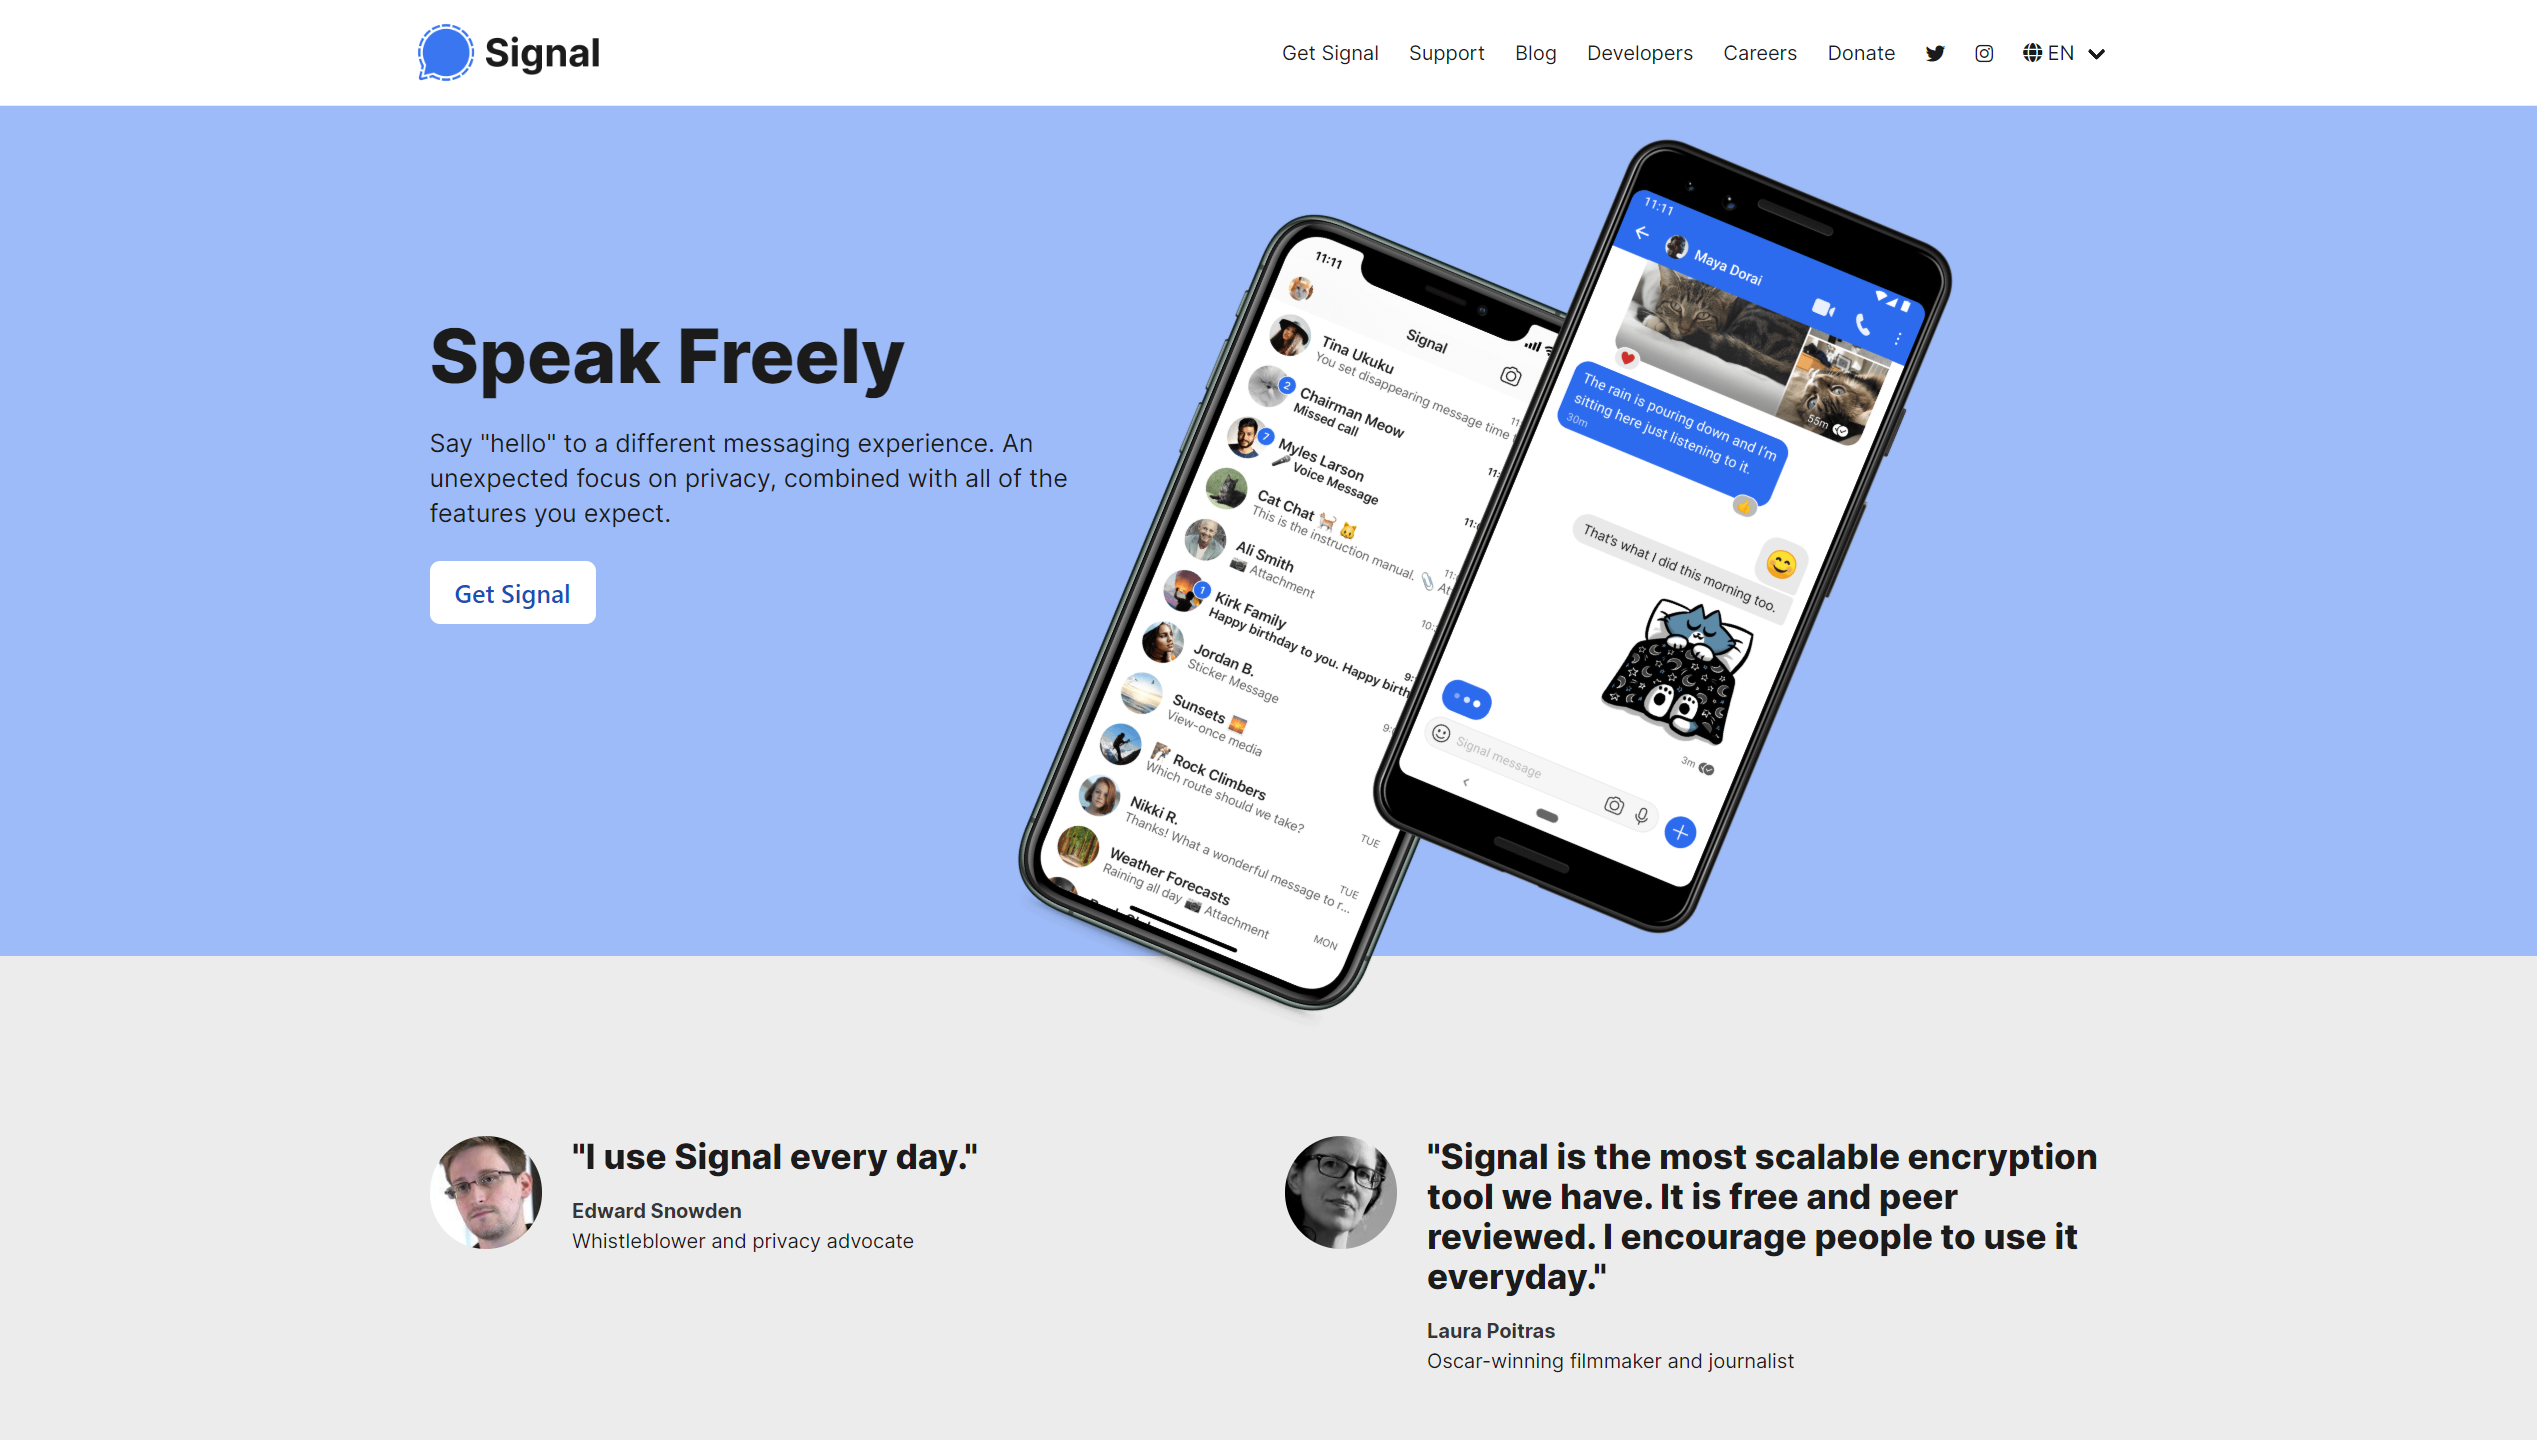
\includegraphics[width=\textwidth]{img/ch-privacy/signal.png}
\end{borderbox}


\section{Virtual Private Networks (VPN)}
Een Virtual Private Network (VPN) cre{\"e}ert een priv{\'e}netwerk op een openbaar netwerk. Het stelt gebruikers in staat rechtstreeks gegevens te verzenden en ontvangen over die openbare netwerken. Toepassingen die over een VPN lopen, kunnen dus gebruikmaken van de functionaliteit, de beveiliging, en het beheer van het priv{\'e}netwerk. Via een VPN zijn online verbindingen niet volledig anoniem, maar de online privacy en veiligheid wordt zeker verhoogd. Om te vermijden dat priv{\'e}gegevens openbaar worden gemaakt, staat een VPN doorgaans alleen geverifieerde toegang op afstand toe. Dit gebeurt met behulp van tunnellingprotocollen en encryptietechnieken.\medskip

\begin{topbox}{\textbf{Top}}
    ProtonVPN biedt uitstekende kosteloze en betaalde VPN-oplossingen die naadloos aansluiten bij de versleutelde e-maildiensten van ProtonMail. 
    \tcblower
    Ga naar \href{https://protonvpn.com/}{ProtonVPN}.
\end{topbox}


\section{Privacy \& beveiliging van internet browsers}
Er zijn uitstekende browsers beschikbaar waarbij de standaard privacy-instellingen zijn aangepast en een paar beveiligings \say{add-ons} zijn ge{\"i}nstalleerd. Houd er echter rekening mee dat geen enkele browser perfect is: elke browser heeft zijn eigen sterke en zwakke punten. Kijk eens naar de favorieten in \href{https://nordvpn.com/blog/best-privacy-browser/}{deze lijst} om de voor jou meest geschikte te vinden en gebruik die in combinatie met met andere tools, zoals een extensie om reclame te blokkeren en een VPN.\medskip

\begin{quotation}
       \textit{\say{If you are not paying for your product, you very well might \emph{\textbf{be}} the product.}}
\end{quotation}

\medskip

Momenteel is Firefox de beste priv{\'e} browser onder de gangbare en bekende browsers met grotere extensie-compatibiliteit en gebruiksgemak. Als je behoefte aan anonimiteit verder reikt of als je toegang wilt tot het dark web, dan zijn Brave (met Tor ingebouwd) of de Tor Browser goede kandidaten.

Onze favoriet is Brave, een open source browser gebouwd door een team privacy-bewuste web-pioniers. Brave is opgericht door de uitvinder van JavaScript en de mede-oprichter van Mozilla. Het is een soepele browser met een heleboel functies, waaronder een ingebouwde adblocker, een wachtwoordbeheerder, trackingbeveiliging en scriptblokkering. Daarnaast kan de verbinding automatisch worden opgewaardeerd van \emph{http} naar \emph{https}, dat veiliger is. Brave belichaamt een nieuwe manier van denken over hoe het web werkt. Ze maken gebruik van microtransacties en hierdoor is het \emph{internet of value} een stap tastbaarder maakt.\medskip

\begin{tipbox}{\textbf{Tip}}
    Brave maakt gebruik van de cryptocurrency BAT, ofwel Basic Attention Token, waarmee de gebruiker zijn favoriete websites kan \emph{tippen} en crypto's kan verdienen gedurende normale internet activiteiten. 
    \tcblower
    Meer weten? Ga naar \href{https://brave.com/urm569}{Brave}.
\end{tipbox}

\section{Alternatieve zoek machines}
Ook wat betreft zoekmachines is de keuze groot. De bekendste is natuurlijk Google. Deze maakt gebruikt van krachtige en intelligente algoritmen (inclusief AI-implementaties) met specifieke zoekresultaten voor de specifieke gebruiker. Deze 'service' heeft uiteraard ook een keerzijde. Het gaat ten koste van de privacy van de gebruiker. Google slaat \emph{alle} gegevens op gebruikt die ook, en weet zoedoende vaak meer over internetgebruikers dan zijzelf. Google houdt praktisch alles bij met betrekking tot zoekopdrachten, clicks, en andere acties via Google-diensten zoals Gmail. Voor iedereen die op zoek is naar meer privacy, zijn er gelukkig goede alternatieven, check \href{https://itsfoss.com/privacy-search-engines/}{deze lijst}.\medskip

\begin{topbox}{\textbf{Top}}
    DuckDuckGo is een zoekmachine-extensie en -applicatie die standaard bij de Brave-browser wordt toegepast en ook in Chrome kan worden gebruikt. DuckDuckGo verzamelt of deelt geen persoonlijke gegevens en slaat de zoekgeschiedenis niet op. Hierdoor hebben ze ook geen gegevens om te verkopen aan adverteerders die je via het internet volgen. Terwijl andere zoekmachines je toch kunnen volgen in de priv{\'e}browsemodus, volgt DuckDuckGo gebruikers nooit.
    \tcblower
    Ga naar \href{https://duckduckgo.com/}{DuckDuckGo}.
\end{topbox}

\section{Back-ups van gevoelige data}
Naast de installatie van een wachtwoord-manager wordt aangeraden tenminste {\'e}{\'e}n kopie van de belangrijkste gegevens op een extra veilige (fysieke) plek op te slaan. Als je om welke reden dan ook de toegang tot jouw computer of mobiele telefoon verliest, kun je vanaf een ander apparaat nog toegang krijgen. Vervolgens kan de wallet in kwestie worden hersteld op basis van de opgeslagen back-up. Het kan nuttig zijn om zoveel mogelijk 'worst case scenario's' te bedenken, zodat alle mogelijke onvoorziene gebeurtenissen gedekt zijn. Enkele voorbeelden zijn zaken zoals brand, diefstal, een computervirus of waterschade.

Door rekening te houden met zulke scenarios ben je altijd goed voorbereidt. Het is bijvoorbeeld niet verstandig om je gegevens alleen maar op te slaan op een notitie-applicatie, computer, cloud-opslag, Google Drive of in een Dropbox. Het risico dat je computer of het gecentraliseerde bedrijf dat deze gegevens bewaart, wordt gehackt en de wachtwoorden worden gestolen, is namelijk niet ondenkbaar.\medskip



\section{Voorkom data-phishing}
Men kan n{\`o}g zoveel maatregelen nemen, uiteindelijk blijft online veiligheid en privacy afhankelijk van de mate waarin gebruikers alert blijven in de online omgeving.

De oorsprong van een hack kan vaak worden herleid tot een persoon die op een link in een e-mail of persoonlijk bericht klikt. Er kan onopzettelijk malware uit een e-mail gedownload worden omdat hij van een collega lijkt te komen. Dergelijke aanvallen worden phishing genoemd. Indien je niet zeker weet hoe phishing eruit zou kunnen zien, blader dan eens door je mailbox voor een scala aan voorbeelden.\medskip

\begin{tipbox}{\textbf{Tip}}
    Klinkt iets te mooi om waar te zijn? Dan is het in 99\% van de gevallen ook zo! Wees extra op je hoede als aan je gevraagd wordt ergens op te klikken of in te loggen en denk altijd aan onderstaande punten!
    \tcblower
    Lees meer op \href{https://www.securitymetrics.com/blog/7-ways-recognize-phishing-email}{Securitymetrics}.
\end{tipbox}
\medskip

\begin{enumerate}[label=(\alph*)]
  \setlength\itemsep{0em}
    \item Instanties vragen nooit gevoelige informatie op via e-mail.
    \item Instanties noemen klanten bij hun naam.
    \item Instanties gebruiken hun eigen, bedrijfsgebonden domeinnamen.
    \item Instanties of bedrijven voeren een correct taalgebruik.
    \item Instanties of bedrijven, crypto-projecten en individuen geven doorgaans geen gratis crypto weg op sociale media of andere platforms.
    \item Instanties of bedrijven zullen mensen niet proberen over te halen om op buttons en links te klikken om belangrijke informatie te achterhalen.
    \item Instanties of bedrijven sturen doorgaans geen ongevraagde bijlagen.
\end{enumerate}



